\documentclass[../../Main/main.tex]{subfiles}
\graphicspath{{\subfix{./Resources/images/}}}

\begin{document}
% Main Body
\chapter{Matter}

\section{What is Matter?}
\begin{easylist}
	# \colorbox{dracPink}{Matter is the “stuff” that makes up everything in the universe.}

	% \Definition{Matter}{Anything that has mass and takes up space.}{\autocite{matter}}

	# Properties of Matter
	## Each specific substance has its own combination of properties that can be used to identify the substance.
	## \highlight{Matter can $\Delta$ it's properties.}\sidenote($\bigstar$)!red!{$\Delta$ means "Change"}
	### Ex. Water is a
	####  Liquid at room temperate
	####  Solid at cold temperatures
	####  Gas at high temperatures
	## Examples:
	### Hardness
	### Texture
	### Flammability
	### Color
	### Shape
	### Temperature

	\bigskip

	This is some text that I want to put a side margin note in for. \sidenote($\bigstar$)!orange!{Test side note}
	\newpage

	% \Definition{Chemistry}{The science that studies what everything is made of and how it changes.}{\autocite{chemistry}}

	\section{Kinds of Matter}

	% Elements
%     |     combine together to get
%     V
% Compounds
%     |     mix together to get
%     V
% Mixtures
\begin{tikzpicture}[>=latex, colorbar arrow/.style={
				shape=double arrow,
				double arrow head extend=0.125cm,
				shape border rotate=90,
				minimum height=5cm,
				shading=#1
			}]
	% Define the 'rect' style for nodes
	\tikzset{rect/.style={draw, rectangle, rounded corners, minimum width=2cm, minimum height=1cm, fill=white}}

	% Nodes for boxes
	\node[rect] (elems) {Elements};
	\node[rect, above=of elems] (cmpds) {Compounds};
	\node[rect, above=of cmpds] (mixs) {Mixtures};

	% Arrows between boxes
	\draw[->, thick] (elems.north) -- (cmpds.south) node[midway, xshift=20mm]{\red{Combine} together to get};
	\draw[->, thick] (cmpds.north) -- (mixs.south) node[midway, xshift=16mm]{\red{Mix} together to get};

	\draw[->] (cmpds.north)--(mixs.south)node[midway, xshift=16mm]{\red{Mix} together to get};
	Define the Starting and Ending RGB Colors
	Start Color (Bottom): RGB(189, 147, 249) -> A purplish color
	End Color (Top):    RGB(255, 121, 198) -> A pinkish color

	\gradientArrow[xpos=-1.5cm, ypos=1.8cm, length=5cm, tailColor=dracGreen, tipColor=dracRed]{Complexity}

\end{tikzpicture}


	# Elements

	% \Definition{Element}{A substance that is made up of only one type of atom.}{\autocite{chemical_elements}}

	## If you break down an element any more, then it just becomes generic \emph{protons}, \emph{neutrons} and \emph{electrons}.
	### It stops behaving like that element
	\begin{itemize}
		\item Ex: If you break down Gold into protons, neutrons and electrons, it is no longer a shiny metal that conducts electricity.
	\end{itemize}
	## Each element has its own symbol
	### Usually the first 1 - 2 letters in the name
	### \highlight{Always CAPITAL\ lowercase if two letters long}
	### Examples
	\begin{itemize}
		\item \highlight{O $\rightarrow$ \underline{O}xygen}
		\item \highlight{He $\rightarrow$ \underline{He}lium}
		\item C $\rightarrow$ \underline{C}arbon
		\item H $\rightarrow$ \underline{H}ydrogen
		\item Al $\rightarrow$ \underline{Al}uminum
		\item Au $\rightarrow$ \marginnote{The latin word for Gold is "\underline{Au}rum", so it still follows the rule, just in a different language.}{Gold}
	\end{itemize}


	# Compounds

	% \Definition{Compound}{A chemical compound is a substance made of two or more different elements joined together by chemical bonds in a fixed ratio.}{\autocite{chemical_compounds}}


	\begin{multicols}{2}
		Ex: Carbon Dioxide ($CO_2$)\\

		\chemfig{%
			\circledatom{dracOrange}{O}=\circledatom{dracBg}{\dracFg{C}}=\circledatom{dracOrange}{O}
		}

		\columnbreak

		Ex: Water ($H_{2}O$)\\

		\chemfig{%
			\circledatom{dracOrange}{O}%
			(-[:-52.25]\circledatom{dracCyan}{H})%
			(-[:232.25]\circledatom{dracCyan}{H})% 180+ 52.5 <-- lower left hydrogen
		}
	\end{multicols}

	% \Definition{Chemical Formula}{A combination of symbols that show the ratio of elements in a compound.}{\autocite{chemical_formula}}

	## Examples\\

	\begin{multicols}{2}

		\begin{itemize}
			\item \(C_{6}H_{12}O_{6}\)
			\item \(NaCl\)
			\item \(CH_{4}\)
			\item \(CO_{2}\)
			\item \(CaCO_3\)
			\item \(Al(OH)_3\)
		\end{itemize}
	\end{multicols}

	# Mixtures

	% \Definition{Mixture}{A substance that is made up of two or more simpler substances. These substances can be chemical elements or compounds. A mixture can be made of liquids, solids, or gases.}{\autocite{mixture}}

	## Ex: Well Water
	### Well water is a mixture because it has minerals, salts, and even dissolved oxygen within it

	\section{Changes in Matter}

	# Physical Changes

	% \Definition{Physical Change}{A type of change in which the form of matter is altered but one substance is not transformed into another. The size or shape of matter may be changed, but no chemical reaction occurs. }{\autocite{physical_change}}

	\begin{figure}[h] % [htbp] are placement options (here, top, bottom, page)
		\centering % Centers the image and caption
		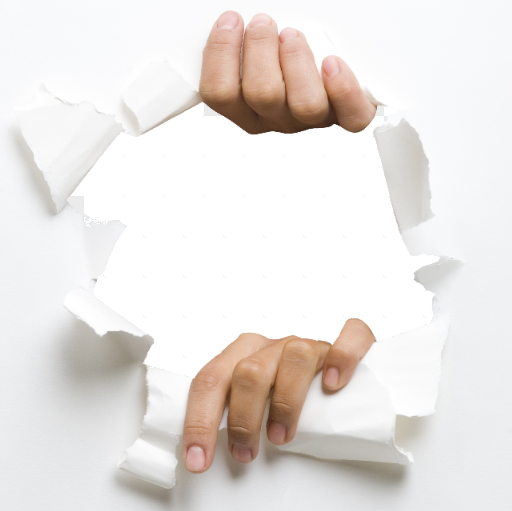
\includegraphics[scale=0.25]{./Resources/Images/rippingPaper.png}
		\caption{Ripping Paper} % The caption text
		\label{fig:example_image} % Optional: label for referencing the figure
	\end{figure}
	## Before it is ripped, it is paper
	## After it is ripped, it is still paper
	### Thus, this is an example of a \emph{physical change.}
	## Other examples
	### Melting Ice
	### Smashing a rock

	\newpage

	# Chemical Changes

	% \Definition{Chemical Change}{A chemical change, a.k.a. a chemical reaction is a change of materials into other materials with different properties. }{\autocite{chemical_change}}

	## \highlight{Chemical changes occur when}
	### \highlight{A substance combines with another to form a new substance.}

	OR

	### \highlight{Chemical decomposition into two or more different substances.}

	## Examples
	\begin{itemize}
		\item Burning Wood
		\item Iron Rusting
		\item Mixing Baking Soda and Vinegar
	\end{itemize}

	\section{Measuring Matter}
	# Mass
	# Weight
	# Volume
	# Density
\end{easylist}

\newpage

\section{Matter Formulas}

\begin{formulaBox}{Density}
	\showFormula{Density}{\center$density = \frac{mass}{volume}$}{\center\unitsDensity}
	\color{dracPurple}\rule{\textwidth}{1.5pt}\color{black}
	\showFormula{Mass}{\center$mass = density \cdot volume$}{\center\unitsMass}
	\color{dracPurple}\rule{\textwidth}{1.5pt}\color{black}
	\showFormula{Volume}{\center$volume = \frac{mass}{density}$}{\center\unitsVolume}
\end{formulaBox}

\begin{formulaBox}{Pressure}
	\showFormula{Pressure}{\center$pressure = \frac{force}{area}$}{\center\unit{atm}}
	\color{dracPurple}\rule{\textwidth}{1.5pt}\color{black}
	\showFormula{Force}{\center$force = pressure \cdot area$}{\center\unit{\newton}}
	\color{dracPurple}\rule{\textwidth}{1.5pt}\color{black}
	\showFormula{Area}{\center$area = \frac{force}{pressure}$}{\center\unit{\centi\meter\squared} | \unit{\meter\squared}}
\end{formulaBox}

\subsection{Gas Laws}

\begin{formulaBox}{Boyle's Law}
	\showFormula{Pressure}{\center$pressure = \frac{force}{area}$}{\center\unit{atm}}
	\color{dracPurple}\rule{\textwidth}{1.5pt}\color{black}
	\showFormula{Force}{\center$force = pressure \cdot area$}{\center\unit{\newton}}
	\color{dracPurple}\rule{\textwidth}{1.5pt}\color{black}
	\showFormula{Area}{\center$area = \frac{force}{pressure}$}{\center\unit{\centi\meter\squared} | \unit{\meter\squared}}
\end{formulaBox}

\begin{formulaBox}{Charle's Law}
	\showFormula{Pressure}{\center$pressure = \frac{force}{area}$}{\center\unit{atm}}
	\color{dracPurple}\rule{\textwidth}{1.5pt}\color{black}
	\showFormula{Force}{\center$force = pressure \cdot area$}{\center\unit{\newton}}
	\color{dracPurple}\rule{\textwidth}{1.5pt}\color{black}
	\showFormula{Area}{\center$area = \frac{force}{pressure}$}{\center\unit{\centi\meter\squared} | \unit{\meter\squared}}
\end{formulaBox}

\begin{formulaBox}{Gay-Lussac's Law}
	\showFormula{Pressure}{\center$pressure = \frac{force}{area}$}{\center\unit{atm}}
	\color{dracPurple}\rule{\textwidth}{1.5pt}\color{black}
	\showFormula{Force}{\center$force = pressure \cdot area$}{\center\unit{\newton}}
	\color{dracPurple}\rule{\textwidth}{1.5pt}\color{black}
	\showFormula{Area}{\center$area = \frac{force}{pressure}$}{\center\unit{\centi\meter\squared} | \unit{\meter\squared}}
\end{formulaBox}

\end{document}
